
Modern avionic systems continue to grow larger in size and complexity, and
state-of-the-art flight control systems can consist of more than a million lines
of code. Lockheed Martin's F22 Raptor contains approximately 1.7M lines of
code~\cite{dvorak2009nasa} and the next-generation F35 fighter is estimated to
comprise 5.7M lines of code.  This trend is not limited to the military arena;
the software content of the Boeing 787 is estimated at 13 million lines of
code~\cite{judas2011historical}.

Concurrently, advancements in networking technology enable increasingly
distributed systems, and network-centric Integrated Modular Avionics (IMA)
architectures are now the industry norm across all aircraft segments, from large
air transport A380~\cite{itier2007a380} to general
aviation~\cite{ananda2009general}.  This integration of multiple aircraft
functions into IMA architectures offers many benefits. Leveraging common
hardware may enable significant SWaP (size weight and power)
reduction. Standardization on hardware platforms may support the improved
optimization of the system obsolescence management. Finally, the ability to
support more cooperation between traditionally federated aircraft functions may
support greater efficiency and safety. The benefits of such integration are
argued in ~\cite{rushby2000partitioning}.

%% However, the increased functionality and higher levels of integration increases
%% system risks in the form of common-mode influences on the host or networked
%% platform and the interaction state space of the hosted functions. New technology
%% and assurance methods could counter these risks.

Industrial architectures often evolve and are usually based on informal
assumptions. By establishing a formal model of the system, we can uncover many
undocumented assumptions. Once formal models are developed, we have found that
the application of formal methods can systematically uncover edge cases and
erroneous behavior that are not otherwise obvious. For example, in our previous
work developing fault-tolerant
protocols~\cite{dutertre2012model,driscoll2012maximizing}, we found that the
application of model checkers is particularly valuable for uncovering erroneous
edge cases in the protocol logic. In~\cite{dutertre2012model}, we further
demonstrated the ability to leverage the formal models developed during protocol
design to generate system-level test cases.

Formal modeling is typically---but not exclusively---used to reason about
behavior. Architectural modeling helps to document and reason about
non-functional properties. Numerous architectural languages, including
AADL\cite{feiler2006architecture}, EAST-ADL~\cite{debruyne2005east},
SLIM~\cite{bozzano2009compass}, and SYSML~\cite{friedenthal2011practical} have
emerged in the past decade. Analysis tools support the models developed using
architectural modeling notations. These tools support many aspects of system
examination from schedulability~\cite{singhoff2005scheduling} analysis to
failure and propagation analysis (HiHOPs~\cite{papadopoulos2011engineering} and
ADAPT~\cite{liu2009reliability}), and automated fault-tree
generation~\cite{li2011method,joshi2007automatic}.

While introducing formal or architectural modeling into a distributed system
development effort can improve the documentation and quality of the system, it
comes at a high cost. In particular, it means there are three separate artifacts
to maintain and keep consistent: the formal model, the architectural model, and
the actual system implementation. Ensuring their consistency is ad-hoc, as each
language has its own syntax and semantics with no connections between them. At
best, the additional effort required to keep the models consistent outweighs the
benefits of increased assurance. At worst, it provides a false sense of
assurance, where the implementation does not satisfy properties specified in
architectural or formal models.

The central thesis of the research described here is that formal models and
analysis is not cost effective unless those models are integrated into the
software development process so that there is one central view of the system and
the models and analysis are directly connected with the software. Without a
formal link through the system refinement and implementation processes, we risk
the \emph{abstraction gap} where implementation details may impact the
assumptions of the higher level abstract model of the system that has been
formally argued. We call the specification that generates models and
implementations an \emph{architectural domain-specific language} (ADSL). The
user needs only to specify the system in one language, and from that, has
multiple ``views'' onto the system.


 %% composable system analysis and verification is primarily achievable through  \emph{apriori} model synthesis and an iterative, generative approach. We believe that the correct modeling paradigm for distributed systems also needs to support different levels of system abstraction and provide an incremental path of system refinement from the high-level  system models to system implementation.  In addition  to meeting the system assurance needs, we also believe that it is necessary to integrate the levels of abstraction and system refinement to ensure that the assumptions made at one level are suitably accounted for or discharged at the lower or higher level. This accounting is especially important when developing formal models to support the architectural claims and fault-tolerance reasoning of distributed systems. Although formal methods technology has improved, current tools are unable to deal with the lower-level details of system implementation due to simplifying abstractions for tractability of analysis and/or scalability limitations. Instead the formal properties of the system architecture or fault -tolerant protocol services are often formally proved using higher level abstract models.  

%% There are two obvious ways to solving the problem of disconnect between
%% different models. One way is to do post-hoc verification each of the three
%% specifications are refinements (abstractions) of one another. Doing so is a
%% monumental undertaking, requiring specifying the semantics of each language and
%% building verification tools to automatically prove refinement. Even if
%% feasible, it does not solve the problem of having to specify a system in
%% multiple languages.

%% The other approach, which we have taken, is to \emph{generate} formal models,
%% architectural models, and implementations from the same specification. 

\begin{figure}
\begin{center}
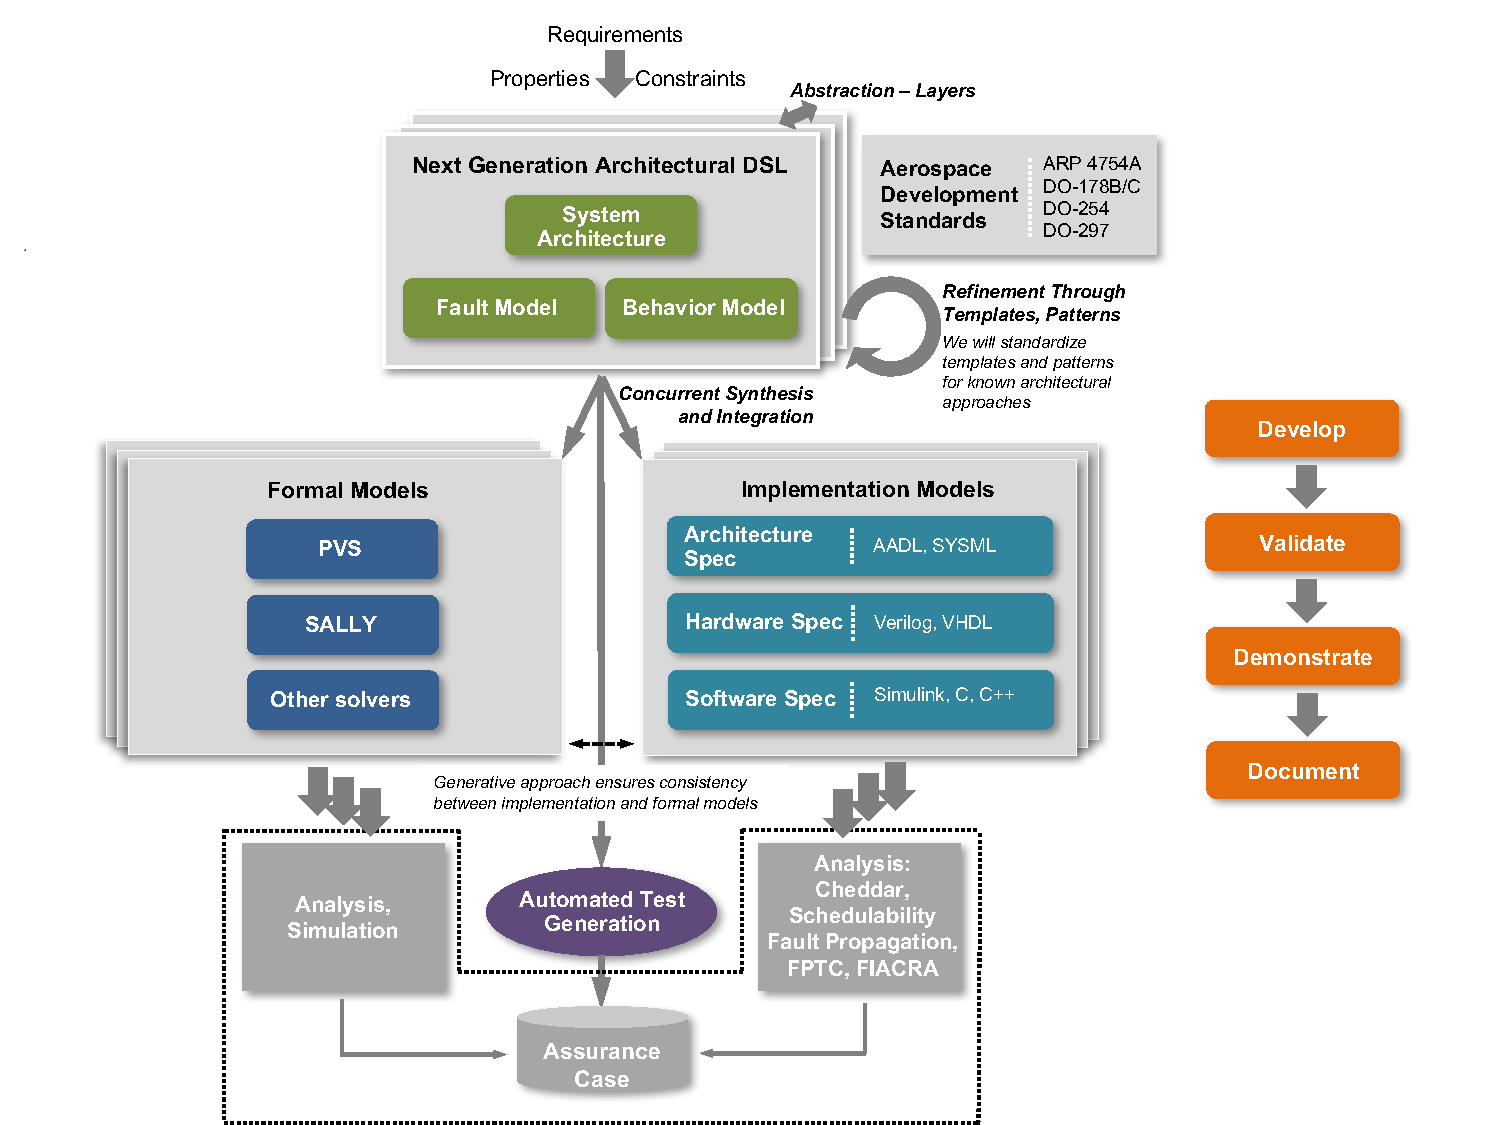
\includegraphics[width=1.0\textwidth]{figures/overall_approach}
\caption{ADSL Approach.}
\label{fig:overall_approach}
\end{center}
\end{figure}

Moreover, while the work we describe here focuses on connecting executable software with formal models for verification, it is in service of our vision for an
architectural workbench as shown in Figure~\ref{fig:overall_approach}. We
envision an ADSL from which multiple analyses are available including

\begin{itemize}
\item Synthesizing formal models (e.g., PVS~\cite{SRI:PVS} for interactive theorem-proving or Sally~\cite{sally} for model checking);
\item Synthesizing architectural models (e.g., SysML~\cite{SysML}, AADL~\cite{feiler06aadl-intro,as5506}), hardware models (e.g., Verilog or VHDL), and software models (e.g., Simulink or C/C++);
\item Automate test generation for system testing from ADSL system models;

\item Integrate into assurance case toolsets (e.g.,~\cite{Rushby05anevidential,CruanesHOS13}) to systematically integrate the
  formal system assurance and associated evidence (e.g., artifacts from analysis
  tools, model checkers, theorem provers, and automated test generation) and
  test artifacts. Ideally, these assurance-cases can be constructed in the context of aerospace development
  standards (e.g., DO-178C~\cite{do178c}, DO-254~\cite{do254}, DO-297~\cite{do297}, ARP-4754~\cite{arp4754}, ARP-4761~\cite{arp4761}).

%% \item Generate low-level implementation, domain-specific languages from system specification  specifically for hardware (e.g., BSV, Chisel, Confluence~\cite{nikhil:bluespec,bachrach2012chisel,TomHawkins:Confluence}) and software (e.g., Ivory, ATOM, Copilot, Scade, Simulink~\cite{ivory:dsl,pike-rv,atom:dsl,esterel:scade,matlab:simulink}) with a path to scoping of directed individual hardware and software component V\&V coverage.
\end{itemize}

\noindent
We have not completed this full integrated vision, but we have made our ADSL makes significant advances toward it. In particular, we address the difficult aspect, which is developing a succinct language for specifying distributed systems with sufficient fidelity to synthesize implementations as well as formal models for verification.

Such a vision touches upon a wide range of research, which we highlight in
Section~\ref{sec:current}, particularly focusing on architectural description
languages and formal analysis tools, our current focus. Earlier, we have
described our language as an \emph{domain-specific} language; the domain we
focus on here are fault-tolerant distributed systems commonly found in aerospace
systems. Toward that end, we outline the concepts that a language specialized
for this domain should imbue. For example, such a language must be able to succinctly allow designer's to specify and reason about different fault models, message-passing constructs, and real-time constraints. We describe these concepts in Section~\ref{sec:towards-adsl}. The concepts drive the design and implementation of the ADSL itself, described in Section~\ref{sec:adsl}. There we introduce the prototype ADSL we have built, which we call LIMA, standing for ``\textbf{L}anguage for \textbf{I}ntegrated \textbf{M}odeling and \textbf{A}nalysis''. We also describe our compilation strategy to both C code and to the input language of Sally, a state-of-the-art model-checker~\cite{sally} that LIMA targets. In particular, the translation to Sally is particularly novel, as we describe an efficient encoding of time, distributed communication, and faults that is amenable to decidable formal analysis. To demonstrate the effectiveness of LIMA, we present case-studies drawn from aerospace systems in Section~\ref{sec:case-studies} that we model in the LIMA and generate executable source code and formal models. These case-studies highlight a unique design feature of the LIMA: it is an \emph{embedded} domain-specific language (EDSL), meaning that it is hosted in a general-purpose programming language. The EDSL approach is common in the programming languages community; we show how it can be used to build powerful new modeling abstractions without introducing new primitives.
 Finally, we present conclusions and future work in Section~\ref{sec:future-work}.


